\section{Data}\label{sec:data}

\subsection{Dataset construction}

To construct price and volume variables I use monthly US customs data from the US Census Bureau between January 2016 through October 2019, which reports monthly import values and quantities at the country-product level using 10-digit Harmonized Tariff Schedule (HTS10) codes by the US Census Bureau to define products, which extend the World Customs Organization's Harmonized System (HS) codes to a more granular level.\footnote{Data is based on values and quantities of imports for consumption, rather than general imports, which may be stored in free trade zones or bonded warehouses without incurring tariff cost, as they are not yet technically in the United States.} 

I estimate the effect of tariffs on prices and volumes at the country ($i$), HTS10 product ($j$), month ($t$) level, consistent with the approach in \textcite{amiti_whos_2020}. Import volume is defined as the dollar value of goods entering the United States. Monthly prices are constructed for each country and HTS10 product by dividing import values by quantities, and prices are defined as the price paid at the border -- the price the US importer pays to the foreign firm. This allows us to study the immediate effect of tariffs, allowing a cleaner identification compared to consumer prices, which would introduce confounders along the supply chain. To calculate tariff-inclusive prices, I multiply every country and HTS10 product pair's monthly price by one plus the corresponding tariff rate for that month. Tariff data is provided by the US International Trade Commission, which defines tariffs for 8-digit Harmonized Tariff Schedule (HTS8) codes, and tariffs at the 8-digit product category level are extended to the 10-digit products within those categories. 

I restrict the sample in several ways. First, I drop petroleum imports due to price volatility that would add excess noise, as done in \textcite{amiti_whos_2020}. Second, I limit the sample only to the first three tariff waves by excluding non-tariffed product categories at the 4-digit level of the Harmonized System (HS). Following \textcite{amiti_whos_2020}, I assume such categories contain comparable products, enabling the study to use non-tariffed HTS10-level products within the same 4-digit category as the untreated group used for comparison. I pool each of these three waves using a relative time scale, where $t=0$ is the month before tariffs are imposed, allowing the model to study the dynamic effects of tariffs across each wave simultaneously. Third, I exclude outliers relative to the median within country-product pairs. Finally, because the US removed tariffs from Canada, Mexico, and Turkey in May 2019, I drop these and subsequent months from the dataset.

I then introduce a trade agreement dummy variable equal to one when a country has a bilateral trade agreement with the United States, using data from the World Bank's Deep Trade Agreements (DTA) database. While the paper initially set out to study whether trade agreement depth -- rather than the existence of a trade agreement alone -- matters, the pattern of the United States' trade agreements makes this impossible, as discussed in Section~\ref{sec:data_descriptive_statistics}. Therefore, I study the effect of agreements in general, and examine whether redefining my study as such changes results in robustness checks. 

I construct the indicator via a concordance of country identifiers between the DTA database and the US Census import data. Because the two sources use different coding systems — the DTA database identifies countries by three-letter alphabetic ISO3 code while the Census data uses a proprietary numeric code — I construct an intermediate lookup table by joining CEPII ISO codes dataset to Census country codes using their shared ISO2 identifier, yielding a crosswalk from ISO3 codes to Census country codes. I then merge the indicator onto the country-level trade agreement pairs using World Bank IDs for trade agreements, and the resulting dataset is matched to the import panel using ISO3 codes.

% Variable definitions
\begin{table}[H]

    \centering
    \caption{Variable Definitions}
        
    \begin{threeparttable}
        
        \begin{tabular}{p{3.5cm} p{7cm} p{4cm}}
            
            \hline
            \textbf{Variable} & \textbf{Description} & \textbf{Source} \\
            \hline
            \\[-1.5ex]

            $\mathbf{i}$ & Subscript indicating country \\[1ex]

            $\mathbf{j}$ & Subscript indicating product \\[1ex]           

            $\mathbf{t}$ & Subscript indicating time (general) \\[1ex]           

            $\mathbf{s}$ & Subscript indicating a particular month \\[1ex]           

            $\textnormal{\textbf{Volume}}_{ijt}$ & Dollar value of monthly imports for country and 10-digit product pairs & US Customs data from the US Census Bureau \\[1ex]

            $\textnormal{\textbf{Quantity}}_{ijt}$ & Monthly import quantities for country and 10-digit product pairs & US Customs data from the US Census Bureau \\[1ex]

            $\textnormal{\textbf{Total tariff rate}}_{ijt}$ & Tariff rate (\%) imposed at the border & US International Trade Commission \\[1ex]

            $\textnormal{\textbf{Price}}_{ijt}$ & Calculated using $\left( \frac{\mathit{Volume}_{ijs}}{\mathit{Quantity}_{ijs}} \right) \times (1 \times \mathit{tariff}_{ijs})$ & Calculation, US Customs data from the US Census Bureau \\[1ex]
            
            $\textnormal{\textbf{Agreement dummy}}_{i}$ & Dummy variable equal to one when a country has a bilateral trade agreement with the US & Constructed using the World Bank's DTA database, CEPII Country Code dataset, and US Customs data from the US Census Bureau \\[1ex]                
            
            \hline
            
        \end{tabular}

    \end{threeparttable}

\end{table}

\subsection{Descriptive statistics}\label{sec:data_descriptive_statistics}

\subsubsection{Tariffs}

The trade war tariffs from 2018 to 2019 raised average tariffs from 1.6 to 5.4 percent, with most of that increase due to tariffs imposed on Chinese goods. As Figure~\ref{fig:average_tariffs} shows, the first three waves raised average tariffs from 1.6 to 2.1 percent. These tariffs applied to \$40 billion of imports. Endogeneity may be an issue to some degree as it is possible the four product categories exposed to tariffs in the selected tariff waves (solar panels, washing machines, steel products, and aluminum products) were chosen for political or geopolitical purposes. However, tariffs' universal application across all countries helps address this and mitigate that risk. 

    % Tariff Distribution
    \begin{figure}[H]
        \centering
        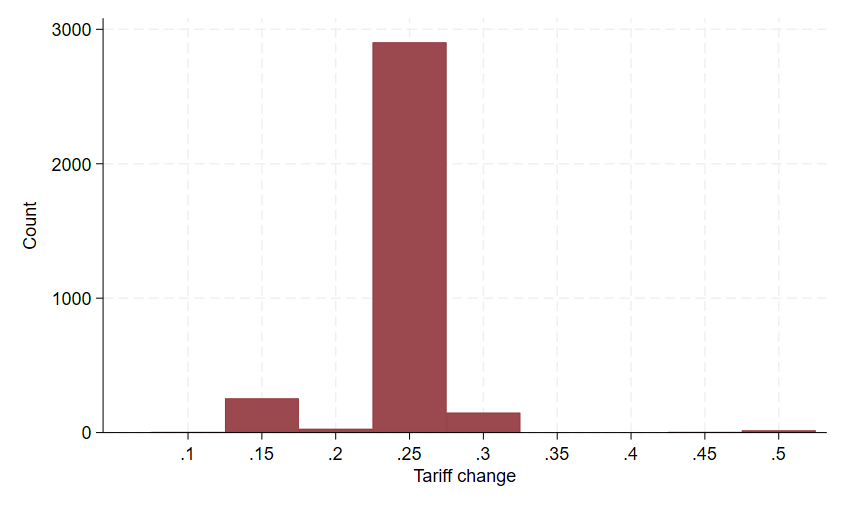
\includegraphics[width=0.85\linewidth]{../Figures/data_figures/tariff_distribution.png}
        \caption{Distribution of tariffs by size in waves 1-3}
        \label{fig:tariff_distribution}
    \end{figure}

    % US ITC tariff data
    \begin{table}[h]
        \centering
        \caption{US ITC tariff data \autocite{amiti_whos_2020}}
        \begin{tabular}{p{3cm} p{2cm} p{2cm} p{2cm} p{2cm} p{2cm}}
            \hline
            \textbf{Variable} & Obs & Mean & Stdev & Min & Max \\
            \hline
            \\[-1.5ex]
            $\textbf{Initial tariff}_{ijt}$ & 23,959,720 & 0.039 & 0.066 & 0 & 3.549 \\[1ex]
            $\textbf{Added tariff}_{ijt}$ & 39,511 & 0.158 & 0.105 & -0.25 & 0.5 \\[1ex]
            $\textbf{Total tariff rate}_{ijt}$ & 23,959,720 & 0.042 & 0.070 & 0 & 3.548 \\[1ex]
            $\textbf{New tariff}_{ijt}$ & 24,449,230 & 0.0016 & 0.0402 & 0 & 1 \\[1ex]
        
        \end{tabular}
    \end{table}

    % Average tariffs - counts: 4, 210, 28, 5, 148, 0,0,4, 16
    \begin{figure}[H]
        \centering
        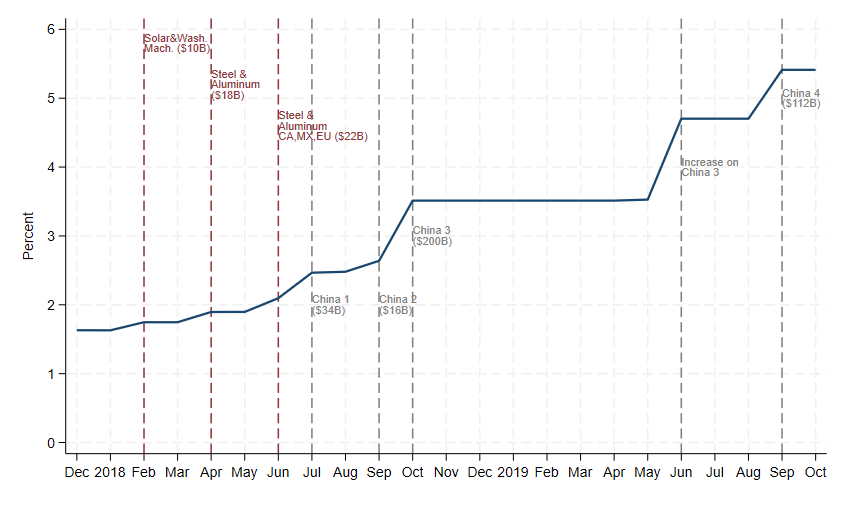
\includegraphics[width=0.85\linewidth]{../Figures/data_figures/average_tariffs.png}
        \caption{Average US tariffs by wave of the 2018-2019 trade war}
        \label{fig:average_tariffs}
        \begin{singlespace}
            \par\noindent\begin{minipage}{0.85\linewidth}
                \footnotesize\textit{Note:} Dashed vertical lines indicate the implementation of each of the eight major waves of new tariffs during the 2018-2019 trade war. This paper studies only the earliest three waves (denoted with maroon lines). Tariffs implemented after the fifteenth of the month counted for the subsequent month. Calculations of average tariffs are based on annual import value across all products in 2017. This graph is sourced from \textcite{amiti_whos_2020}
            \end{minipage}
        \end{singlespace}
    \end{figure}

The United States imposed tariffs relatively consistently in these first three waves, with a modal 25\% tariff applied to nearly 3,000 country and 10-digit product pairs.  

\subsubsection{Trade Agreements}

    % US trade agreements: chart
    \begin{figure}[H]
        \centering
        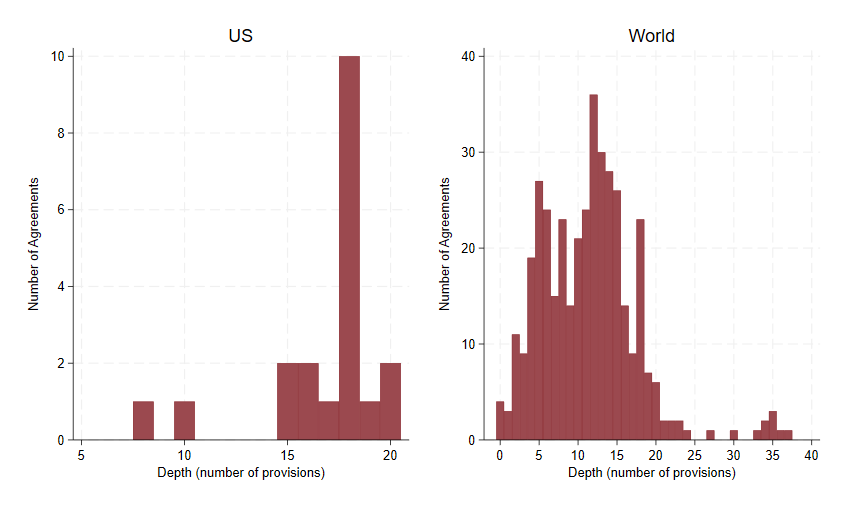
\includegraphics[width=0.85\linewidth]{../Figures/data_figures/us-global_tradeagreements_hist.png}
        \caption{US and Global trade agreements by depth, 2024}
        \label{fig:us-global_trade_agreements_chart}
    \end{figure}

\textcite{mattooTradeCreationTrade2022} define the deepest trade agreements as those with legally enforceable provisions in 20 or more policy areas beyond WTO requirements. Applying this threshold to the US sample would restrict the treated group to NAFTA and USMCA --- effectively, Mexico and Canada alone. Lowering the threshold to 10 legally enforceable provisions, which \textcite{mattooTradeCreationTrade2022} classify as medium-depth, expands the sample to 19 of the 20 countries with which the US has a bilateral trade agreement; only Jordan falls below this cutoff. Any intermediate threshold would be arbitrary, and given the clustering of US agreements between 15 and 20 provisions (Figure~\ref{fig:us-global_trade_agreements_chart}), results would be highly sensitive to the chosen cutoff. I therefore redefine the treatment variable as a binary indicator for whether a country has any bilateral trade agreement with the US, and interpret results accordingly. The original question --- whether deeper trade agreements mitigate tariff shocks --- is examined in robustness checks that vary the depth threshold.

Figure~\ref{fig:us-global_trade_agreements_chart} also shows that the global distribution of trade agreements is substantially shallower than the US distribution. Two implications follow. First, the depth effect could be studied in contexts with greater variation across countries. Second, because US agreements are uniformly deep relative to the global distribution, the resilience effects identified in this paper cannot be extrapolated to trade agreements in general.

\begin{table}[H]
    \centering
    \caption{Sample composition matrix (country-product pairs)}
    \begin{tabular}{l c c c}
        \hline\hline
        & \textbf{Tariffed} & \textbf{Non-tariffed} & \textbf{Total} \\
        \hline
        \textbf{Deep} & 1,280 & 2,387 & 3,667 \\
        & 6.4\% & 11.9\% & 18.3\% \\
        \textbf{Non-deep} & 5,355 & 10,989 & 16,344 \\
        & 26.8\% & 54.9\% & 81.7\% \\
        \hline
        \textbf{Total} & 6,635 & 13,376 & 20,011 \\
        & 33.2\% & 66.8\% & 100\% \\
        \hline\hline
        \multicolumn{4}{l}{\footnotesize\textit{Note:} Count of country-product-month observations = 249,123.}\\
    \end{tabular}
\end{table}

\subsubsection{Trade}

    \begin{figure}[H]
        \centering
        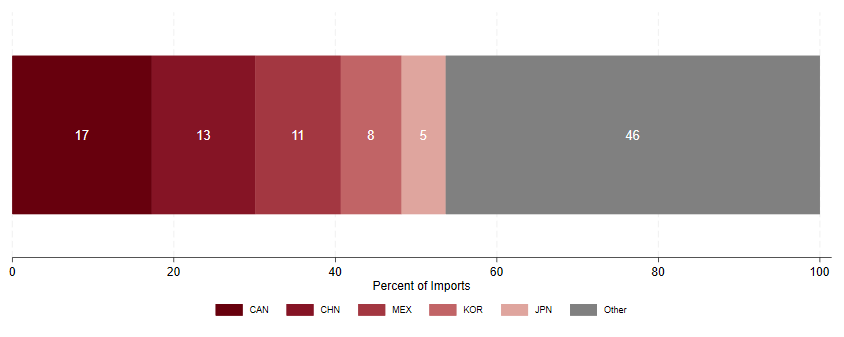
\includegraphics[width=0.75\linewidth]{../Figures/data_figures/total_imports_bycountry_stacked.png}
        \caption{Total US Imports by Source Country, 2017}
        \label{fig:total_imports_bycountry_stacked}
    \end{figure}

    \begin{figure}[H]
        \centering
        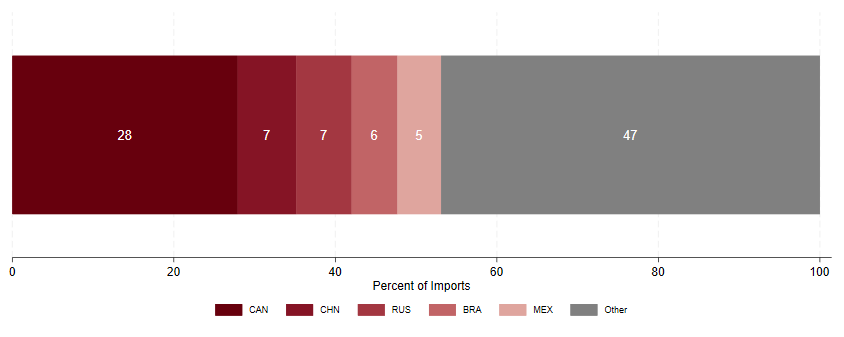
\includegraphics[width=0.75\linewidth]{../Figures/data_figures/steel_imports_bycountry_stacked.png}
        \caption{US Steel Imports by Source Country, 2017}
        \label{fig:steel_imports_bycountry_stacked}
        
        \begin{singlespace}
            \par\noindent\begin{minipage}{0.75\linewidth}
                \footnotesize\textit{Note:} Figures \ref{fig:total_imports_bycountry_stacked} and \ref{fig:steel_imports_bycountry_stacked} are based on the sample of products tariffed in the first three waves at the HS4 level. $N = 249{,}123$ observations at the country-product-month level.
            \end{minipage}
        \end{singlespace}

    \end{figure}

Figures \ref{fig:total_imports_bycountry_stacked} and \ref{fig:steel_imports_bycountry_stacked} show the source composition of US imports in 2017, the pre-tariff baseline year. Across all goods, Canada (17\%), China (13\%), and Mexico (11\%) are the three largest suppliers, with Korea (8\%) and Japan (5\%) rounding out the top five; the remaining 46\% is distributed across 149 other countries. The steel-specific composition differs markedly: Canada accounts for 28\% of steel imports while China supplies only 7\%, consistent with \citeauthor{amiti_whos_2020}'s (\citeyear{amiti_whos_2020}) observation that China is a relatively minor steel supplier to the US market. Russia and Brazil each contribute 7\% and 6\% respectively, with Mexico at 5\%, with the remaining 47\% distributed among 107 other countries. The relative absence of China and relative diversity of suppliers motivates the paper's focus on waves 1–3 of the tariff sequence rather than the China-specific Section 301 waves.